%!TEX root=../protocol.tex	% Optional
% How can WebAssembly (compiled from Rust) in comparison to javascript improve performance in metrics like execution speed or file-size in web-based applications?

\section{Introduction}
Over the last years the usage of web-based application drastically increased \cite[cf.][]{stackoverflow:survey}. The success of \gls{node} marked a turning point in how to build modern applications and web-sites. Instead of developing different native programs for different targets like a Windows-based computer, one web-application is created and ported to different target systems. Frameworks like \gls{electron} or \gls{react:native} enforce this process.

This ``write once, run anywhere'' approach seems like a logical next step to do. But it has one particular drawback: performance. Web-based applications are simple HTML-sites backed with a lot of JavaScript code for logic and more. And here lies the problem. JavaScript was never meant for this.

JavaScript was developed in the 1990s to add interactivity to static web-pages.It was primarily aimed at designers for light \gls{dom}-manipulation and should co-exist with \glspl{java:applet}, which were planned to perform the business logic of the web-application. Java-Applets featured many fundamental design flaws, like requiring a plugin in the browser in order to work, that many programmers used JavaScript in their web-applications instead, because it just worked \cite{js:history, wasm:explanation, javaapplet:history}.

For the last two decades JavaScript was the only reliable way to program on the web. Since 2015 the WebAssembly team, initiated by Luke Wagner at Mozilla and Ben Titzer at Google Munich, worked on creating a new low-level binary format to provide a faster alternative to JavaScript. In other words, a Java-Applet that works. In November 2017 \gls{mozilla} announced that WebAssembly is supported in all major browsers. \cite{wasm:revolution, wasm:support}.  

\section{WebAssembly}

\subsection{General}
WebAssembly (abbreviated \textit{Wasm}) is not a typical programming language. It is primary a binary instruction format, it defines and specifies guidelines how compiled code should look like. The code itself is written mostly in a system-level programming language like C++ or Rust (see next \hyperref[sec:rust]{section}) which is compiled to WebAssembly with the help of a \gls{llvm}-backend. The compiled WebAssembly output can be loaded by a browser that decodes and compiles it to native machine-code, which is later executed \cite{wasm:basics, wasm:howandwhy}.

This approach helps WebAssembly to be \textit{efficient} and \textit{fast}, the main goals of the format. Efficiency is achieved by using an binary format. A binary file is always smaller than a textual file. This helps to keep file-size relatively small. A further benefit of the format is that parsing and optimisation is done while building the WebAssembly output. Therefore, when using WebAssembly in the browser no costly optimisation is needed to generate native high-performance machine code. The execution speed, the fast-aspect of WebAssembly, is mostly based on the used programming language and build tools. WebAssembly compiled from C++ or Rust is way faster in solving algorithms than JavaScript in comparison. This is explainable by the stark differences in the design and concept of the languages. The \hyperref[sec:performance]{performance} section will go deeper into details later.

\newpage

Although WebAssembly is a binary format, it can be defined as a programming language because it features its own syntax and structure. Every WebAssembly binary output (\textit{wasm}) can be transcribed to a textual, assembly-like format called WebAssembly Text Format (\textit{wat}) and vice-versa. This means a WebAssembly program could be programmed without a typical programming language like C++, but instead with assembly code in the \textit{wat}-format. This however is not the recommended way. Writing code in assembly is much more time-demanding because of its syntax. This makes complex programs also harder to maintain. The intention of the \textit{wat}-format is to have a textual representation of the code, when viewing the loaded WebAssembly binary in the browser. This enables the ability of debugging. The textual representation can be used to set breakpoints for the debug-process, which would be impossible with binary code. It also makes sense for WebAssembly to feature an own textual format, in order to be independent from the used source language \cite{wasm:bringthewebtospeed}.

The following demonstrates how an simple algorithm in C++ looks like when compiled to WebAssembly and transcribed to the textual representation:
\begin{listing}
\noindent
\begin{minipage}[t]{0.49\textwidth}
\begin{code}[]{c++}
int factorial(int n) {
  if (n == 0)
    return 1;
  else
    return n * factorial(n-1);
}
\end{code}
\end{minipage}
\begin{minipage}[t]{0.24\textwidth}
\begin{code}[]{lisp}
20 00
42 00
51
04 7e
42 01
05
20 00
20 00
42 01
7d
10 00
7e
0b
\end{code}
\end{minipage}
\begin{minipage}[t]{0.25\textwidth}
\begin{code}[]{bash}
get_local 0
i64.const 0
i64.eq
if i64
    i64.const 1
else
    get_local 0
    get_local 0
    i64.const 1
    i64.sub
    call 0
    i64.mul
end
\end{code}
\end{minipage}
\caption{C++ source code - Wasm format - Wat format \cite{wasm:wat}}
\label{lst:wasm-code}
\end{listing}

The binary output is not human readable. Therefore the \textit{wat}-format exist. It features similarities to Assembler, but it has distinct differences. WebAssembly is executed in a \gls{stackmachine} virtual machine in the browser. The design of the language reflects this usage. Reading the \textit{wat}-format is not that difficult, if known what to look for. The general concept is very simple. Every new value is pushed to a stack. When performing operation, the latest value or values are used and consumed, thereby creating a new value. 

The next listing is included as a guide to help with reading and understanding the \textit{wat}-format.


\begin{listing}
\hspace{1cm} Code \hspace{3cm} Stack \hspace{4cm} Explanation \vspace{-0.5cm} \\\\
\noindent\rule{\textwidth}{0.6pt} \vspace{-0.5cm}
\begin{code}[]{bash}
get_local 0      #   |            | A            # Push first parameter         
i64.const 0      #   | B          | A            # Push constant with value 0
i64.eq           #   |            | eq(B,A)      # Call equals with latest 2 values
if i64           #   |            | eq(B,A)      # If latest 2 values are equal
    i64.const 1  #   |            | C            # Push constant with value 1
else             #   |            | eq(B,A)      # If latest 2 values are not equal
    get_local 0  #   |            | A            # Push first parameter
    get_local 0  #   | B          | A            # Push first parameter
    i64.const 1  # C | B          | A            # Push constant with value 1
    i64.sub      #   | B-C        | A            # Subtract the latest 2 values
    call 0       #   | func0(B-C) | A            # Call itself with latest value
    i64.mul      #   |            | func0(B-C)*A # Multiply the latest 2 values
end              #   |            |              # Return latest value
\end{code}
\caption{Reading Wat}
\label{lst:wat-code}
\end{listing}

\label{sec:rust}
\subsection{Working with Rust}
The concept and basics of WebAssembly were covered in the previous section. As mentioned earlier WebAssembly relies not on a single programming language, instead any programming languages with support can be used.
This work specialises on the programming language \textit{Rust} to give greater insight into the topic. 

Rust was chosen because its one of the languages that fits perfectly into the concept of WebAssembly. This is no coincidence. WebAssembly features no built-in garbage collector, this is a problem for languages like Java or Go, that rely on it, but not for system-languages like Rust or C++. One of the benefits of Rust over C++ is its sophisticated compiler. The Rust compiler detects common errors like dangling \glspl{pointer} (pointers that do not point on valid objects) while compiling and aborts the process if such problems are detected. The C++ compiler is not capable of this. This overall means that a successfully compiled WebAssembly program from Rust is less likely to have basic errors. This is very helpful because debugging is not that easy with WebAssembly and for now only supported in the WebAssembly Text Format.

Another advantage of Rust is its support. Rust is strongly community-driven, but it is also backed by the organisation behind the initial WebAssembly proposal and the Firefox web browser: Mozilla. With the resources and knowledge of Mozilla, Rust has the best chances to become a prominent language of the web with the help of WebAssembly \cite{rust:intro}.

The Rust WebAssembly project, called \textit{rust-wasm}, is divided in many sub-projects that are used together to make Rust fit for WebAssembly. The most important ones are \textit{wasm-pack} and \textit{wasm-bindgen} \cite{rust:wasm}.

\newpage

\textit{Wasm-pack} is used to compile Rust code to WebAssembly. It uses \textit{wasm-bindgen} to generate a JavaScript file that is needed to call functions from WebAssembly. This all is wrapped up in a directory, in default called \textit{pkg}, that can be used in a NodeJS project as a \gls{nodemodule}. For starters it is recommended to use the \textit{ \href{https://github.com/rustwasm/wasm-pack-template}{wasm-pack-template}} which is a minimal, pre-configured project best suited for starting to work with Rust and WebAssembly in NodeJS.

\textit{Wasm-bindgen} is used to create a bridge between WebAssembly and JavaScript. This is needed at the moment because there is no way to call WebAssembly functions directly from HTML. Therefore, JavaScript is needed as ``glue-code'' to make WebAssembly work. This is somewhat a design choice from the WebAssembly team that positions WebAssembly as an addition to JavaScript especially where high-performance is needed. Wasm-bindgen also allows to import JavaScript functions to WebAssembly which makes it possible to use them like native functions in the source code. The following example imports the \textit{alert}-functions from JavaScript and exports a custom \textit{alert}-function called \textit{greet} from the WebAssembly module.
\begin{listing}
\begin{code}[]{rust}
use wasm_bindgen::prelude::*;

// Import the `window.alert` function from the Web.
#[wasm_bindgen]
extern "C" {
    fn alert(s: &str);
}

// Export a `greet` function from Rust to JavaScript, that alerts a
// hello message.
#[wasm_bindgen]
pub fn greet(name: &str) {
    alert(&format!("Hello, {}!", name));
}  
\end{code}
\caption{Rust source-code for WebAssembly \cite{rust:wasmbindgen}}
\label{lst:rust-wasm-bindgen}
\end{listing}
The through \textit{wasm-pack} compiled and packaged WebAssembly program can be then imported like a Node Module in a NodeJS project and called like a normal function.
\begin{listing}
\begin{code}[]{javascript}
import { greet } from "./wasm_module_pkg";

greet("World!");
\end{code}
\caption{Calling a WebAssembly function through JavaScript \cite{rust:wasmbindgen}}
\label{lst:js-wasm-bindgen}
\end{listing}

\newpage

\label{sec:performance}
\section{Performance}
This section describes how WebAssembly can be used to speed up web-applications and what performance gains one can expect.
\subsection{Theoretical advantages}
First, the question needs to be asked what advantages WebAssembly has as a format in in terms of execution speed compared to JavaScript. Note, this sections assumes that a system-level programming language like Rust is used as a basis for the WebAssembly module.

The process of creating executable code out of JavaScript source code is quite long. The plain text needs to be parsed first into a data structure called ``abstract syntax tree''. Then the JavaScript engine can compile the data structure into machine code. While compiling, the engine has also the important task of optimising the written code. This means that the ``quality'' of the compiled code is strongly depended on the JavaScript engine of the browser. Better optimised code is tied to longer compilation times that want to be short as possible. WebAssembly eliminates the steps of parsing and optimisation when loaded by the browser engine. A WebAssembly module is already pre-compiled and optimised before used in the browser. The engine only needs to decode the WebAssembly module and compile the binary format to the corresponding target system. This last compilation step of WebAssembly requires no optimisation, its just a porting process \cite{wasm:howandwhy}. 

JavaScript relies on a garbage collector for memory management. That means that a process inspects what memory areas are used and which ones are unused and frees them if so. This helps to eliminate memory inconsistencies and also takes the responsibility of writing manual memory operations in the code from the programmer. This however has the drawback that a heavy-weighted process for the garbage collector is needed to be executed in the browser engine all the time. It also makes the general execution speed of a program unpredictable because the garbage collector can always perform an operation in the midst of program call. In comparison WebAssembly relies on a single linear memory. Memory management is tied to the written code, not an automated garbage collector. Rust for example still needs its own memory allocator shipped in WebAssembly, but this is needed for memory management of the linear memory WebAssembly features and is not related to a garbage collector. WebAssembly with its manual memory management can therefore be faster and much more reliable than JavaScript. But this is only true, if the manual memory management is cleanly implemented. Rust as a language helps to make memory management safer through concepts like \gls{rust:ownership} that translate well to WebAssembly. 

\newpage

\subsection{Practical Benchmarks}
To enforce full transparency, all programs used for testing can be found here: \url{https://github.com/kurbaniec-tgm/WebAssembly-Paper}.

\subsubsection{Fibonacci}
The first benchmark portrays a heavy computational use-case. In short, the 30th number of the Fibonacci sequence is determined. For referenence, the Fibonacci number is the sum of the two preceding numbers: $F_n = F_{n-1} + F_{n-2}$.

The following shows the algorithms determining the Fibonacci number. On the left the implementation for Rust and WebAssembly is displayed, on the right the JavaScript version.

\begin{listing}
\noindent
\begin{minipage}[t]{0.57\textwidth}
\begin{code}[]{rust}
fn fibonacci(n: u32) -> u32 {
    match n {
        0 => 1,
        1 => 1,
        _ => fibonacci(n - 1) + fibonacci(n - 2),
    }
}
\end{code}
\end{minipage}
\begin{minipage}[t]{0.4\textwidth}
\begin{code}[]{javascript}
function fibonacci(num) {
    if (num <= 1) return 1;
    return fibonacci(num - 1) + fibonacci(num - 2);
}
\end{code}
\end{minipage}
\caption{Fibonacci source code - Rust/Wasm - JS \cite{wasm:wat}}
\label{lst:wasm-code}
\end{listing}

\vspace{-0.2cm}
For testing, every algorithm was executed ten times per run. The Rust version was tested with Rust Nightly on a Windows 10 based machine. The WebAssembly and JavaScript versions were tested on the same machine in the Chrome- and Firefox-browser.

\begin{listing}
\begin{center}
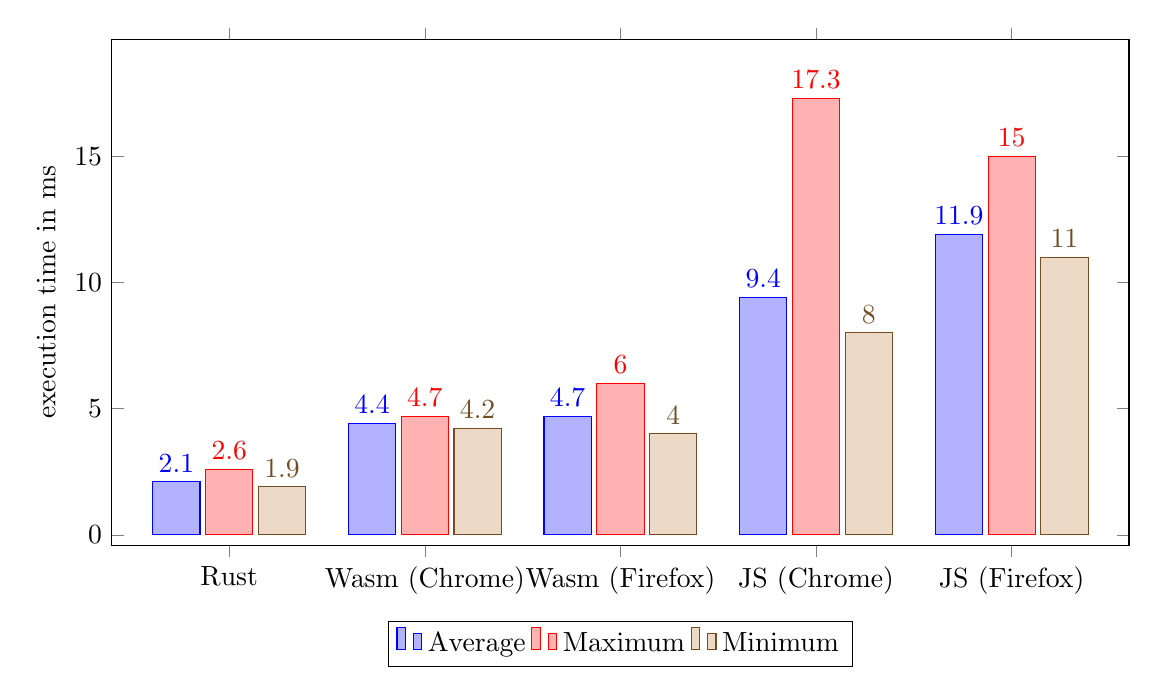
\begin{tikzpicture}
\begin{axis}[
    ybar,
    height=8cm, width=14.5cm,
    bar width=0.6cm,
    enlargelimits=0.15,
    legend style={at={(0.5,-0.15)},
      anchor=north,legend columns=-1},
    ylabel={execution time in ms},
    symbolic x coords={Rust,Wasm (Chrome),Wasm (Firefox), JS (Chrome), JS (Firefox)},
    xtick=data,
    nodes near coords,
    nodes near coords align={vertical},
    ]
\addplot coordinates {(Rust,2.1) (Wasm (Chrome),4.4) (Wasm (Firefox),4.7) (JS (Chrome),9.4) (JS (Firefox), 11.9)};
\addplot coordinates {(Rust,2.6) (Wasm (Chrome),4.7) (Wasm (Firefox),6.0) (JS (Chrome),17.3) (JS (Firefox),15.0)};
\addplot coordinates {(Rust,1.9) (Wasm (Chrome),4.2) (Wasm (Firefox),4.0) (JS (Chrome),8.0) (JS (Firefox), 11.0)};
\legend{Average,Maximum,Minimum}
\end{axis}
\end{tikzpicture}
\end{center}
\caption{Fibonacci Benchmark}
\label{lst:fibonacci-benchmark}
\end{listing}

The results show expected behaviour. The Rust implementation is more than double as fast as the WebAssembly one. This is understandable because the Rust version runs on the local and WebAssembly runs in a virtual stack-machine in the browser powered by the local machine. But the important part is that the WebAssembly version is more than double as fast as the JavaScript version. Both versions run in virtual machines in the browser, but WebAssembly as a format is way more efficient to be consumed and executed by the browser engine than JavaScript. What also is visible is the consistent performance of WebAssembly in comparison to JavaScript. This can by explained with interference from JavaScript's garbage collector.  

WebAssembly as a binary format should be smaller than a JavaScript file in theory. The sole Fibonacci algorithm in JavaScript is a 117 Bytes large file. In comparison, the WebAssembly output is 862 Bytes. The executable Rust output is the largest with 3.37 Megabytes.

\begin{listing}
\begin{center}
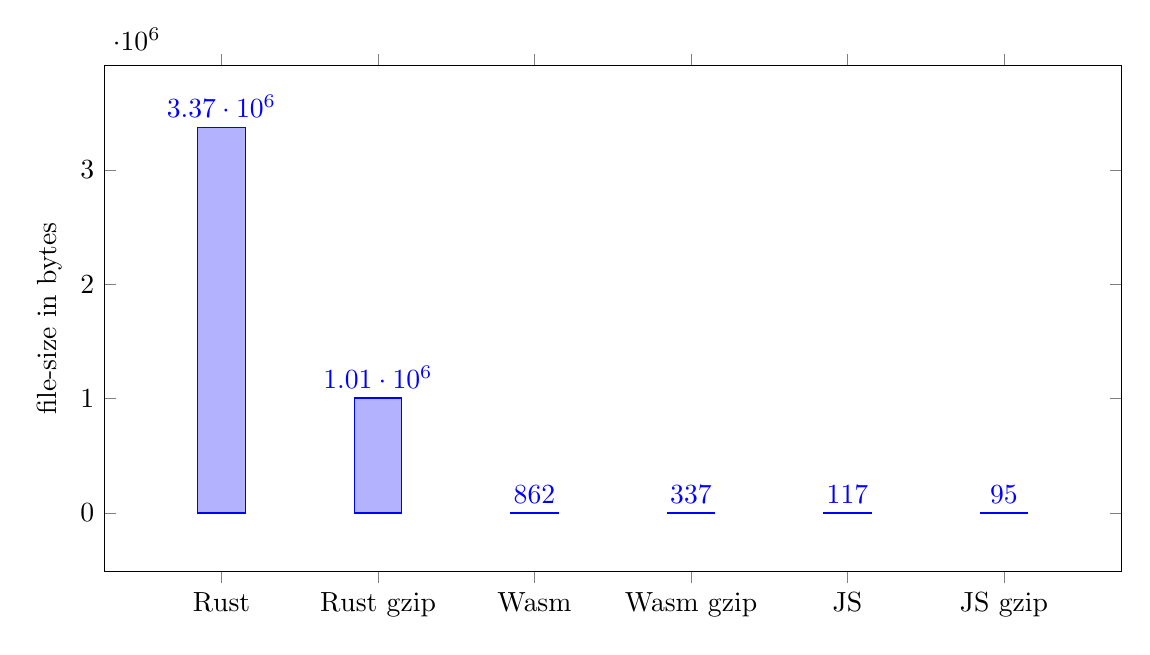
\begin{tikzpicture}
\begin{axis}[
    ymin=0,
    ymax=3400000,
    ybar,
    height=8cm, width=14.5cm,
    bar width=0.6cm,
    enlargelimits=0.15,
    legend style={at={(0.5,-0.15)},
      anchor=north,legend columns=-1},
    ylabel={file-size in bytes},
    symbolic x coords={Rust,Rust gzip,Wasm,Wasm gzip, JS,JS gzip},
    xtick=data,
    nodes near coords,
    nodes near coords align={vertical},
    ]
\addplot coordinates {(Rust,3373261) (Rust gzip,1005336) (Wasm,862) (Wasm gzip,337) (JS,117) (JS gzip,95)};
\end{axis}
\end{tikzpicture}
\end{center}
\caption{Fibonacci file-size}
\label{lst:fibonacci-filesize}
\end{listing}

This stark differences can be explained by the fact that is is not a true one-to-one comparison. The JavaScript file features only the algorithm with no additional code. The WebAssembly module features the algorithm with needed additions like a memory allocator (examples use the smallest one possible called \textit{wee\_alloc}) that are needed for execution. The Rust executable features the algorithm, the main-test program and full bindings for the targeted host machine. Also, a fully fledged memory allocator is included. But most of the time resources are shared compressed over the internet. With the compress utility \textit{gzip} we can determine how large the files are when transferred efficiently. WebAssembly's binary format is perfect for compression, we can reduce the size to one third of the original one. JavaScript's textual files do not benefit greatly from compression and are only reduced slightly. Therefore, it can be expected that a long algorithm or algorithms will probably be smaller in WebAssembly than JavaScript. The overhead of the needed additions in WebAssembly will be at some point smaller than the inefficiency of a textual file \cite{wasm:allocator, rust:wasmfilesize}.

\subsubsection{Multihreaded Markdown-Parser}
The second benchmark portrays a mor real-word example with the inclusion of multithreading, in other words parallel processing. The task is simple, a \gls{markdown}-file should be parsed to a native HTML-output. To achieve higher performance, the file is split already split in three parts that can be individually converted and then concatenated together at the end.

At the moment WebAssembly features no native thread implementation. There is already a proposal and some early implementation, but further developed slowed down since the discovery of Meltdown and Spectre \cite[cf.][]{wasm:threads}. Nonetheless, WebAssembly can achieve parallel processing in the same manner as Javascript: Web Workers. A Web Worker is an object that runs a JavaScript-file (and WebAssembly) in a distinct thread. 

TODO

\begin{listing}
\noindent
\begin{minipage}[t]{0.45\textwidth}
\begin{code}[]{rust}
use comrak::{markdown_to_html, ComrakOptions};

...
let mut options = ComrakOptions::default();
options.unsafe_ = true;
markdown_to_html(&text, &options)
...
\end{code}
\end{minipage}
\hspace{1cm}
\begin{minipage}[t]{0.45\textwidth}
\begin{code}[]{javascript}
import('./bower_components/showdown/dist/showdown.js').then(showdown => {
    ...
    const converter = new showdown.Converter();
    converter.setFlavor('github');
    const html = converter.makeHtml(text);
    ...
}
\end{code}
\end{minipage}
\caption{Markdown-Parser source code - Rust/Wasm - JS}
\label{lst:wasm-code}
\end{listing}

\begin{listing}
\begin{center}
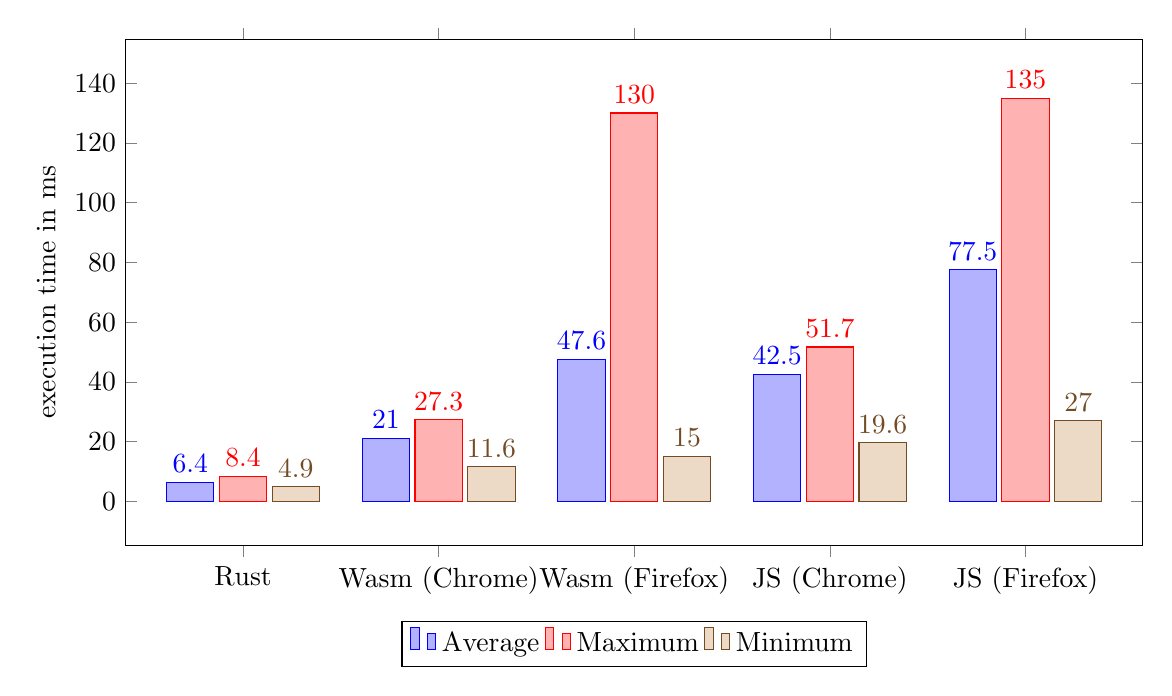
\begin{tikzpicture}
\begin{axis}[
    ybar,
    height=8cm, width=14.5cm,
    bar width=0.6cm,
    enlargelimits=0.15,
    legend style={at={(0.5,-0.15)},
      anchor=north,legend columns=-1},
    ylabel={execution time in ms},
    symbolic x coords={Rust,Wasm (Chrome),Wasm (Firefox), JS (Chrome), JS (Firefox)},
    xtick=data,
    nodes near coords,
    nodes near coords align={vertical},
    ]
\addplot coordinates {(Rust,6.4) (Wasm (Chrome),21.0) (Wasm (Firefox),47.6) (JS (Chrome),42.5) (JS (Firefox), 77.5)};
\addplot coordinates {(Rust,8.4) (Wasm (Chrome),27.3) (Wasm (Firefox),130.0) (JS (Chrome),51.7) (JS (Firefox),135.0)};
\addplot coordinates {(Rust,4.9) (Wasm (Chrome),11.6) (Wasm (Firefox),15.0) (JS (Chrome),19.6) (JS (Firefox), 27.0)};
\legend{Average,Maximum,Minimum}
\end{axis}
\end{tikzpicture}
\end{center}
\caption{Multihreaded Markdown-Parser Benchmark}
\label{lst:markdown-benchmark}
\end{listing}

\section{Conclusion}

TODO

\subsection{Future Outlook}
wasi?


%\makefig{images/logo-right.png}{height=2cm}{
%    Mit Beschreibung und Label  % (Optional)
%}{
%    fig:caption-label           % (Optional)
%}


